\chapter{Часть 2}

\section{Призраки над Каиром}

Ранним утром 4-го ноября 1969 г., два «Фантома» с ревом взлетели с авиабазы Рефидим на Синае и исчезли в западном направлении. Они пронеслись над Суэцким заливом, огибая паруса рыбацких лодок. Над пустыней, которую вскоре сменила водная гладь рукавов и зеленые равнины дельты Нила. Обогнули радиомачты, позиции ПВО, разбитые «Скайхоками», "перепрыгнули" ЛЭП, поднявшись до 50 метров над землей — и вот они уже в предместьях Каира. Без единого выстрела. Прямо под ними вырастают пирамиды Гизы и Сфинкс.

«Прямо как на картинках» - думает Давид Яир, штурман ведущего «Фантома», когда его машина взмывает на трёхкилометровую высоту под вой сирен и суматоху вокруг египетских радаров ПВО, заметивших гостей в самом сердце зоны ПВО Каира. И — пикирует вниз. Давид заметил, как Шмуэль Хец, его пилот и командир 201-й эскадрильи "Фантомов" передвинул РУД вправо и вперёд, почувствовал, как дополнительная масса топлива была впрыснута в форсажные камеры двигателей, образуя длинные оранжевые хвосты за их самолётом. Как самолёт резко ускорился и превысил скорость звука. Впереди лежал Миншат аль-Баккари — правительственный район Каира и резиденция Насера. За фонарем изолированной от внешних шумов кабины летчики не слышали, как по улицам людского муравейника внизу проносится громоподобное эхо, разбивающее вдребезги тысячи окон, бьющее по барабанным перепонкам и сеющее панику.

Египтянам нечем было ответить на такую наглость. Этот рейд не был первым: в июне пара «Миражей» фоторазведки случайно прошла на сверхзвуке над Гелиополисом. Тогда это стоило погон командующему ВВС Египта, Мохаммеду Багдади. Сейчас — совсем другая история. Это не Гелиополис, это Каир, столица. И это не «Миражи», а «Фантомы», у них два двигателя — и значительно более мощных. И это сотни МиГов и зенитных ракет египтян, охраняющих сердце Египта. И они беспомощны ...

\begin{figure}[h!tb] 
	\centering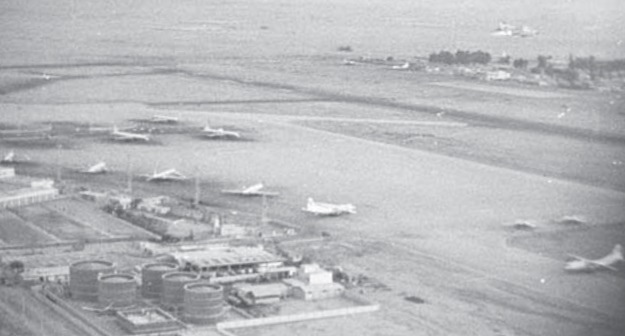
\includegraphics[scale=0.4]{Dolina_2/Aub6T35ajmo.jpg}
	%	\label{fig:scipion} % Unique label used for referencing the figure in-text\end{document}
	%	%\addcontentsline{toc}{figure}{Figure \ref{fig:placeholder}} % Uncomment to add the figure to the table of contents%----------------------------------------------------------------------------------------
	\caption{"Фантом" Шмуэля Хеца (в правом верхнем углу) взлетает на форсаже. Фото оператора вооружений второго «Фантома» Ахикара Эяля. 4 ноября 1969. Фото из книг Шломо Алони.}%	CHAPTER 2
\end{figure}

К концу 1969-го война набирала обороты. 13-го сентября 1969 генерал Хаим Герцог на пресс-конференции для журналистов сказал: «Линия фронта с Египтом не обязательно проходит только по Суэцкому каналу. Она охватывает весь Египет». Это был очевидный намёк Насеру: если война будет продолжаться, то совсем не так, как ты хочешь. «Мишенью становится весь Египет, а не только солдаты Насера в районе Канала». Теперь у израильтян были не только перехватчики — «Миражи» и устаревающие «Самбады». У них было нечто совсем новое.

За восемь дней до той пресс-конференции Герцога, в пятницу 5-го сентября 1969, за несколько минут до начала Шаббата на авиабазе Хацор, в присутствии высокопоставленных приглашённых, приземлилась первая четвёрка израильских «Фантомов». На них быстро закрасили американские опознавательные знаки, и нанесли местные: шестиконечную синюю Звезду Давида на белом фоне.

На Святую землю прибыл новый король. «Фантом» (или «Курнасс», "кувалда" на иврите) был по-настоящему "народным самолётом" — деньги на покупку первой партии собирали по всему Израилю. «Дайте своему сыну Фантом!» — кричали газеты. И вот самый дорогой истребитель в мире наконец прибыл. Это был прорыв - «Фантом» не уступал «Миражу» в воздушных боях, но был на голову, на порядок лучше в качестве ударного самолёта. Он мог доставить тонны бомб в любую точку Египта — а затем показать пилотам египетских МиГов, почему попытка им помешать может стать для них последней.

11-го ноября экипаж «Фантома» № 08 69-й эскадрильи (Эхуд Ханкин — Ахикар Эяль) удостоился чести быть первым, встретившим МиГ-21 в воздухе. И первым, сбившим его.

17-го ноября «Фантом» №04 станет первым сбитым (отличилась иорданская ПВО). Экипаж (Эхуд Ханкин — Шауль Леви) будет спасен; они погибнут через 3 года, на второй день Войны Судного дня, возглавляя атаку на позиции сирийских ПВО на Голанских высотах.

В общем, слова Герцога не были пустыми угрозами. В сентябре 1969 у израильтян появился отличный способ их воплощения. Но почему вопрос об ударах по тылу встал так поздно — ведь с начала активных боев прошло больше полугода?

В начале войны на истощение Израиль старался воздерживаться от любых действий, которые могли бы привести к эскалации войны. Бомбардировки - только ответные, рейды за канал - только точечные. Выполнили задачу - ушли. ВВС работали только в зоне Суэцкого канала - реакция и египтян, и американцев на атаки египетского тыла была непредсказуема. К тому же было совершенно непонятно, может ли Насер (и готов ли он) остановить войну. К концу 1969-го г. стало понятно, что нет, не готов. К тому же в сентябре 1969-го г. Ицхак Рабин, тогда - посол Израиля в США, отправил в Иерусалим небезызвестную телеграмму, в которой оценил вероятность отказа США от помощи Израилю в случае эскалации боевых действий как маловероятную, развязав еврейскому государству руки.

На следующий день, на совещании в генеральном штабе было принято решение перенести основную тяжесть бомбардировок из района Суэцкого канала - вглубь Египта. Разведка (в лице главы АМАН и уроженца Москвы Аарона Ярива) предположила, что тяжесть таких бомбардировок станет для Насера непомерной, и он наконец решит закончить войну, которую сам развязал. ВВС была поставлена задача - пробить “коридор” в поясе египетских ЗРК в районе Канала. Через 24 часа заслон из восьми египетских батарей ЗРК перестал существовать! Путь вглубь страны фараонов был открыт.

А дальше — дело техники. Идеальным самолётов для “стратегических” (в масштабах Ближнего Востока) бомбардировок был именно“Фантом”. Он мог нести втрое больше бомб, чем “Миражи”, и вдвое - чем “Скайхоки”, к тому-же “Фантомам” не требовался эскорт - при случае их пилоты с удовольствием могли ввязаться в бой с МиГами. “Фантомы” прорывались к цели на малой высоте, практически не оставляя времени для того, чтобы организовать перехват силами истребителей. Израильтяне имели большое разнообразие маршрутов - с севера, со стороны моря, с востока - через Сохненскую и Заафранскую долины. Они появлялись внезапно, били больно, и так же быстро исчезали. Как призраки.

\section{Голиаф прибывает}

20-го декабря 1969 года, в обстановке строжайшей секретности, первые советские Ан-12, приступили к доставке в Египет, на авиабазу Кайро-Уэст, разобранных советских МиГов и их лётчиков отдельной разведывательной эскадрильи. Авангарда советских регулярных войск в Египте. Для советских пилотов всё это было непривычным. Представьте себе — из привычных +15 вы отправляетесь в адскую жару, слепящую пустыню со скорпионами, змеями, мухами и прочими прелестями. Им предстояло ещё очень многое узнать о местных жителях и их нравах.

Зарулили на стоянку. Выгрузились. Выдохнули. Осмотрелись. Начали разгружаться. И - под вой сирен бросились в песок. Через секунды небо над авиабазой взорвалось разрывами десятков снарядов. И тут же - над самыми крышами капониров пронеслась пара железных птиц с таким знакомым хищным профилем «Фантомов».

“Хель Ха-Авир приветствуют русских лётчиков”. Какая там, говорите, секретность?

Египетские С-75 отстрелялись “вдогонку” несколькими ракетами, после чего египтяне радостно сообщили, что сбили один “Фантом”. Правда, через некоторое время их радость поубавилась: оказалось, что вместо израильского самолёта под раздачу попал собственный буксировщик мишеней Ил-28 - впрочем, египтяне всё равно радовались как дети — наконец-то им удалось сбить хоть кого-то! Чем наводили советских пилотов на очень неприятные размышления о качествах новых союзников...

В самом конце декабря 1969 г. 10 советских генералов в сопровождении огромной свиты прибыли в Египет, чтобы лично осмотреть и выбрать будущие позиции ЗРК и аэродромы базирования авиации. Возглавлял их сам Маршал СССР Батицкий - главком войск ПВО и личность в этих самых войсках весьма легендарная. Во время этой поездки произошел забавный эпизод: встречавшему советских офицеров Насеру все присутствующие были представлены поименно, называя и звание, и должность. Когда Батицкий представлял запмолита будущей советской дивизии, генерал-полковника Халипова, Насер не понял смысл его должности и переспросил - а что это? Батицкий вышел из положения красиво - “это духовный отец” - ответил он.

Такие «Духовные отцы» были в каждом советском подразделении в Египте. Зачастую их присутствие создавало бОльшие проблемы - догматичные и зашоренные, эти люди иногда пытались навязать свое мнение в общении с египтянами. В худшем случае они вдохновенно вещали о преимуществах прогрессивного социалистического строя и всеобщего равенства. Как правило - людям, родившимся с серебряной ложкой и вышедшим из потомственной аристократии. Египтяне крутили пальцами у виска, но слушали.

Весь январь в Египет прибывал авангард советского “экспедиционного корпуса” в лице 35-й отдельной разведывательной эскадрильи - летчики, техники, офицеры и их самолёты. На подходе были зенитно-ракетные дивизионы (их доставят морем) и 135-й полк на МиГ-21.

К 1-му февраля 1970 г. отдельная эскадрилья полковника Юрия Настенко заступила на боевое дежурство на аэродроме Джанкалис. Операция по спасению Насера началась.

\section{Расцвет над Египтом}

Прибытие советских самолётов было очень кстати. В начале января израильтяне после нескольких дней разведки приступили к ударам по египетским тылам.

Серию операций назвали «Приха» (“расцвет” на иврите). Операция “Приха-1” (7 января 1970) - представляла собой комбинированный удар по нескольким целям: пара “Фантомов” 201-й эскадрильи отбомбилась по школе операторов ЗРК С-75 в районе Хелуана, пара 69-й - по учебному лагерю египетских коммандо под Александрией, четверка “Скайхоков” из 115-й - по штабу 2-го египетского армейского корпуса в Тель эль Кабир, в районе Дельты. Египтяне не успели хоть как-то отреагировать, все цели были уничтожены. Налет произвел на египтян достаточно гнетущий эффект — не столько из-за его последствий и большого числа жертв, не только местных. Хуже было другое. Египтяне просто не понимали, как противостоять таким налётам.

В Тель эль Кабир погиб советник командира пехотной бригады полковник Михаил Кальченко. Первый погибший «руси асири» в новом 1970-м году. И очень, очень далеко не последний.

Через шесть дней всё повторилось - “Скайхоки” 109-й эскадрильи атаковали военный лагерь в районе Дельты, “Фантомы” из 201-й - базу снабжения в Тель эль Кабир. Эффективность ударов превзошла все ожидания - и теперь было решено атаковать чаще и больше. “Приха” стали типовыми операциями ВВС. Сначала -“Миражи” фоторазведки подтверждают объект из банка целей. Потом - “Фантомы” на малой высоте просачиваются через египетское ПВО и уничтожают её.

«Скайхоки» окончательно перестали привлекаться к ударам по египетскому тылу — теперь туда летали только «Фантомы» и «Миражи». 18 января — новый налет, бомбардировка складов боеприпасов в Хелуане. Вторичные детонации в результате огромного пожара на складах продолжались несколько часов после атаки, сея панику в ближайших городах. В огне погибло огромное количество артиллерийских снарядов — их запас пришлось срочно пополнять в СССР. А ещё во время этой бомбардировки израильтяне похоронили последнее детище Вилли Мессершмитта — H-300 Helwan, попытку сделать собственный самолёт, первый разработанный в арабской стране. «Фантомы» уничтожили ангар, в котором хранились первые несколько прототипов.

23 января — «Фантомы» бомбят склады недалеко от гражданского аэропорта Каира. Пассажиры прекрасно видели взрывы и беспомощность военных, снова паника. В тот же день, в ходе операции «Родос», израильтяне атаковали укрепленный остров Шедуан в основании Суэцкого залива. Египтяне потеряли убитыми и пленными больше 100 солдат, включая роту коммандос. Израильтяне — троих. Ночью египтяне послали пару Ил-28 отбомбиться по захваченному острову — безуспешно.

28 января — снова. «Фантомы» атаковали Даншур, склады и школу операторов ПВО, а заодно — здания штаба 6-й моторизованной дивизии в пригороде Каира. Здание было полностью разрушено, под обломками погибли больше ста египетских военных, включая командира дивизии и его заместителя, трое гражданских и двое дивизионных советников — полковник Иван Огибенин погиб на месте, полковник Николай Власенко через 2 дня умер от ожогов в госпитале в Каире. С ними же погиб и их переводчик, лейтенант Зияддин Юсубов. Ещё пятеро советников было ранено. Израильтяне знали, что в штабе есть «хабиры» — но не стали отменять атаку.

После этого налёта, в Каире была введена светомаскировка. Египетская столица погружалась в серый мрак и уныние. Барабаны войны, до этого громыхавшие где-то далеко, теперь стучали в двери каждого египтянина. «Ограниченная война в районе Канала» как-то внезапно распространилась на всю страну.

Почему египтяне не пытались как-то противостоять налётам? Они честно пытались. Проблема была в том, что получалось очень так себе. В начале 1970-го года советники, оказавшиеся на позициях ПВО в районе Канала нередко обвиняли египтян в трусости — они нередко просто покидали позиции при появлении израильских самолётов. «Стреляйте по ним, — говорили советники. — Сбивайте их». Прагматичные египтяне просто сбегали — шансов у батареи С-75 против летящих на высоте 20-40 метров «Фантомов» не было. Ствольная зенитная артиллерия не успевала обстрелять такую быструю цель — так что возможность противостоять налётам израильтян стремилась к нулю. Да, из СССР уже поставили первые ПЗРК (одним из таких был сбит «Скайхок» Ниссима Ашкенази в 1969-м году), но израильтяне просто поменяли тактику. Теперь они чаще бомбили методом «кела» («праща») — говоря по-русски, с кабрирования, не входя в зону поражения ПЗРК и ствольной артиллерии. Так и продолжалось:— СССР поставлял Египту новые батареи, Египет размещал их в районе Канала; у Израильтян часто уходило меньше дня на их уничтожение. Египтяне просили новое оружие. СССР поставлял его ...

В воздухе картина была не сильно лучше. Чаще всего, египетские самолёты просто не успевали подняться на перехват «Фантомов» — подлётное время нередко составляло считанные минуты. Время, необходимое для того, чтобы поднять истребители — не меньше пяти (у египтян, команды из СССР справлялись быстрее). Окей, не получается перехват с земли - по рекомендации советников начали дежурить в воздухе. Получилось лучше. Несколько раз египетские самолёты всё же успевали перехватить атакующие «Фантомы» - как правило, всё заканчивалось для египтян достаточно плохо. В таких ситуациях главное задачей пилотов «Фантомов» было успеть сбить египтянина до того момента, как к ним “на помощь” придут коллеги из эскадрилий Миражей - например, так получилось 8 февраля, во время “Прихи-8”. Авием Селла (просто запомните это имя), замкомэска 69-й эскадрильи, ввязался в бой с преследующим его МиГ-21, лидером пары. Египтянин увернулся от “Спэрроу” и пары “Декеров” (“Шпага”, название AIM-9D в Израиле) - но ввязался в ближний маневренный бой с “Фантомом” и был быстро сбит пушкой. Возможно, кто-то жестоко обманул египетского лётчика, убедив его в превосходстве МиГ-21 в ближнем маневренном бою. Достать второй МиГ Селла не успел - через несколько секунд тот оказался жертвой прибывшего “Миража” Авраама Салмона. Оставшиеся египтяне предпочли не ввязываться в бой.

\begin{figure}[h!tb] 
	\centering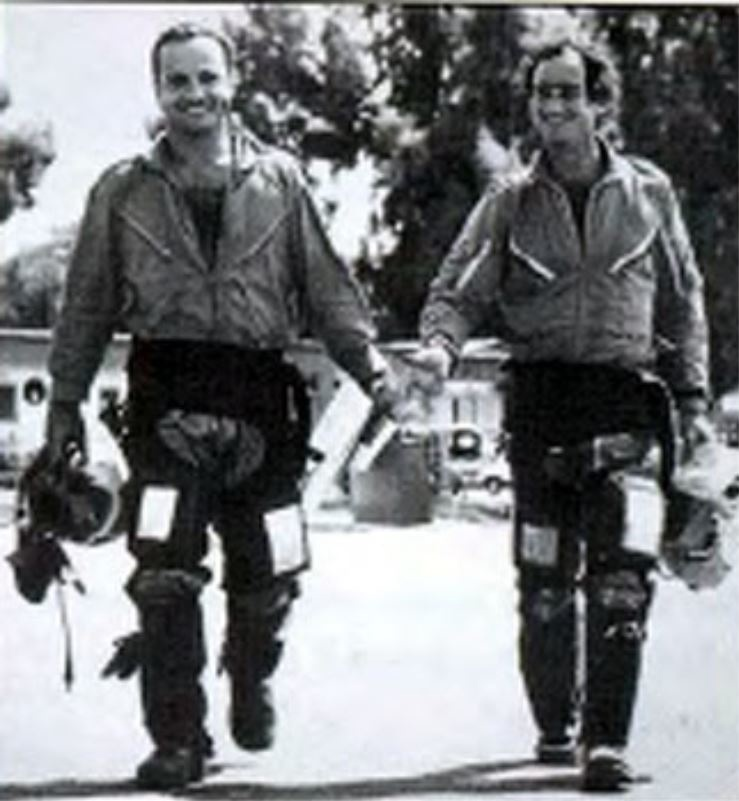
\includegraphics[scale=0.4]{Dolina_2/OXgUBXELWoU.jpg}
	%	\label{fig:scipion} % Unique label used for referencing the figure in-text\end{document}
	%	%\addcontentsline{toc}{figure}{Figure \ref{fig:placeholder}} % Uncomment to add the figure to the table of contents%----------------------------------------------------------------------------------------
	\caption{Авием Селла, Авраам Шалмон (справа)}%	CHAPTER 2
\end{figure}

Советники сначала недоумевали — во Вьетнаме результаты были другими. Но так и противник у Египта был другим — не американские «сухопутные» лётчики, готовившиеся к большой войне и перехвату ракетами за пределами видимости, а потому - слабо обученные ближнему маневренному бою. На израильских «Фантомах» летали ветераны «Миражей» — умные, прагматичные и злые. Американский пилот готовился к совсем другой войне, летал во Вьетнаме 100 вылетов — и отправлялся домой. Израильский — летал, пока его не собьют, или пока не уйдёт на повышение. Справедливости ради, второе случалось чаще, чем первое.

\section{Две большие разницы}

Здесь надо сказать пару слов, почему «вьетнамская» тактика — как у лётчиков, так и у ПВО, не работала на Ближнем Востоке.

Во Вьетнаме американцы использовали, в первую очередь, свою гигантскую воздушную мощь — налеты легко могли производиться совершенно любыми силами, от четырех до сотни машин. Низкая точность регулярных ударов со средних высот компенсировалась огромной массой сбрасываемых бомб. Не справились два звена - отправим шесть. По пути нескольких собьют — окей, потери допустимы. В таких условиях, особенно до появления у американских ВВС достаточно эффективных средств радиоэлектронной борьбы и развития тактики противодействия ЗРК, комплексы С-75 действительно показывали себя хорошо.

\begin{figure}[h!tb] 
	\centering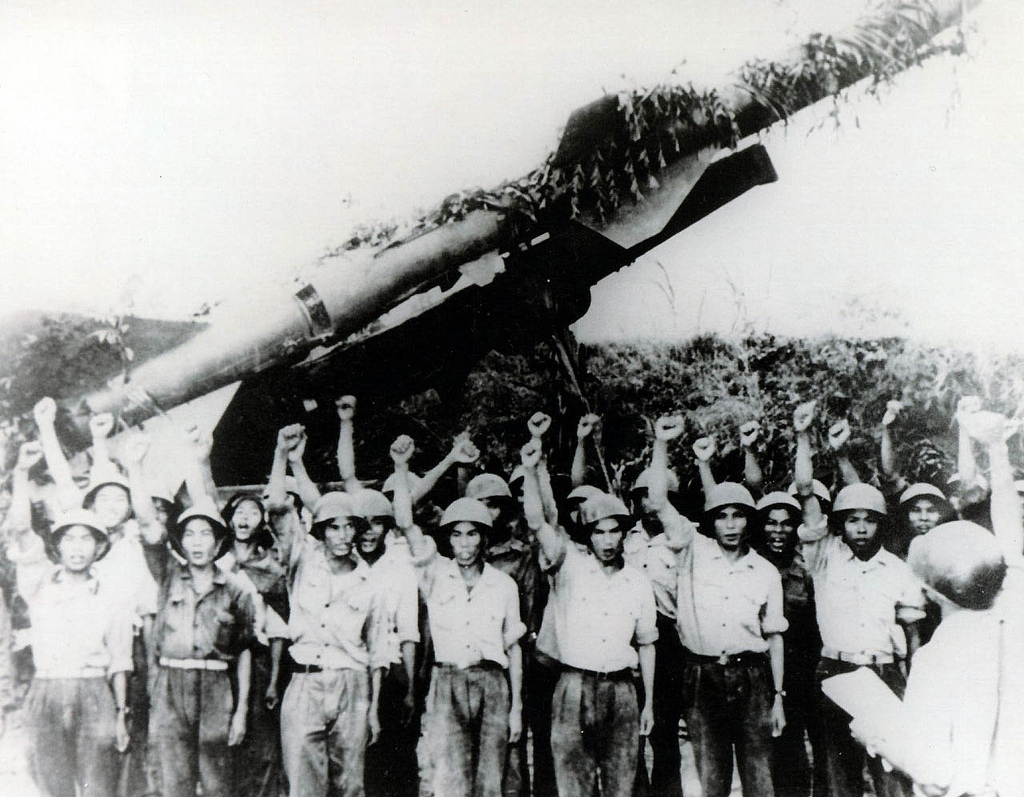
\includegraphics[scale=0.4]{Dolina_2/5BWa6P70FCk.jpg}
	%	\label{fig:scipion} % Unique label used for referencing the figure in-text\end{document}
	%	%\addcontentsline{toc}{figure}{Figure \ref{fig:placeholder}} % Uncomment to add the figure to the table of contents%----------------------------------------------------------------------------------------
	\caption{ЗРК С-75 во Вьетнаме}%	CHAPTER 2
\end{figure}

\begin{figure}[h!tb] 
	\centering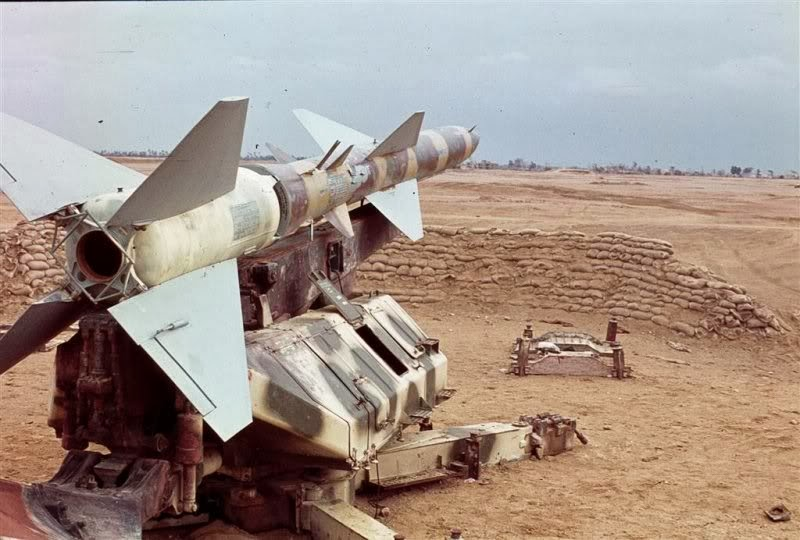
\includegraphics[scale=0.4]{Dolina_2/F8dlw3qe7jg.jpg}
	%	\label{fig:scipion} % Unique label used for referencing the figure in-text\end{document}
	%	%\addcontentsline{toc}{figure}{Figure \ref{fig:placeholder}} % Uncomment to add the figure to the table of contents%----------------------------------------------------------------------------------------
	\caption{ЗРК С-75 в Египте}%	CHAPTER 2
\end{figure}

Лётчики же действовать во «вьетнамском» стиле, то есть как авиация ПВО, египтяне не могли. Не хватало координации, да и противник позволял подойти к себе незамеченным исключительно редко. Гораздо чаще засады подразумевала израильская тактика — но она как раз была рассчитана скорее на тактическую внезапность появления самолётов в бою, чем на «вьетнамский» пуск ракеты с последующим быстрым выходом из боя с уходом на малые высоты. К тому-же в то время подготовка к ближнему маневренному воздушному бою у американских и израильских лётчиков отличалась на порядок. Американцы только к концу 1960-х осознали масштаб провала в обучении пилотов и начали его исправлять. Разумеется, быстро изменить гигантскую структуру ВВС они не могли. Флотские лётчики справились быстрее, но тоже не сразу.

В отличие от Вьетнама, на Ближнем Востоке в конце 1960-хне было бомбардировок со средних высот, массы самолётов и регулярности маршрутов и времени ударов. Не было и американских контейнеров РЭБ, они появились на год позже. Был «моц» - фольга, которую ствольная артиллерия забрасывала, чтобы создать проблемы египетским РЛС. Были «Скайхоки», которые носили эту самую фольгу в воздушных тормозах. И всё. «Голь на выдумки хитра» - израильтяне за неимением большого парка «Фантомов» были вынуждены изобретать новые тактики, действовать нестандартно, не «по-американски». Довольно забавно после этого читать, что в ВВС Израиля служили опытные лётчики, прошедшие Вьетнам. В то время разница в «классе» была такова, что израильтяне легко могли сами учить американцев.

То есть израильские пилоты того времени были, вероятно, наиболее подготовленными строевыми лётчиками в мире.

Вообще, читать наши источники о воздушных сражениях войны на истощение весьма любопытно. Участие советских частей в них описано совершенно великолепно, последовательно и красочно. Но как только разговор заходит об израильских ВВС — складывается впечатление, что читаешь сборник анекдотов про Рабиновича. В них с завидной постоянностью, из года в год, из книги в книгу циркулируют одни и те же сомнительные истории. Казалось бы - в Израиле давно рассекретили всё, что можно рассекретить, война на истощение описана буквально по дням, а иногда - по минутам. Бери, сравнивай. Но нет, зачем, мы будем цитировать советские байки и прочие «ранее закрытые источники».

Возьмём, к примеру, информационно-методический сборник ЦМВС РФ, публикация «Победы и неудачи советских летчиков и ракетчиков в небе над Египтом» 2013 года. Писал, к слову, начальник Музея ПВО, историк Юрий Кнутов. Казалось бы, уже изданы «Призраки над Каиром» Дани Шалома, разменяли второй десяток «оспреевские» сборники Алони, уже поработали Том Купер, Дэвид Николле, Амир Сегев, Дэвид Лединцер, Авирам Баркаи написал свою восхитительную «От имени небес». Уже существует "объединение каирских историков", Авиноам Мисников уже завел свой чудесный сайт. Информации не просто море — её океан. На любой вкус.

Но что мы видим вместо этого? Правильно, «израильская авиация, пилотируемая, в том числе и успевшими повоевать во Вьетнаме американскими летчиками, регулярно бомбила территорию Египта». Какие, к черту, американские лётчики? На каком они, интересно, разговаривали языке?

Читаем дальше, и видим там … 25 (!) потерянных «Миражей» в боях только с египтянами в 68-70 годах! Я всё понимаю, пропаганда это дело такое ... но ведь 50 лет уже прошло. В реальности их было 10 (5 над Египтом, 2 над Сирией и 3 в авариях), потеря целой эскадрильи (25 машин) в боях только с одной АРЕ была бы для израильтян образца 70-го года катастрофой.

Вообще, об израильских ВВС принято писать или в хвалебном, или в уничижительном тоне. «Промежуточные» варианты можно встретить куда реже. Скорее всего причина в том, что израильтян в СССР никогда не рассматривали как серьёзного противника. Не из-за недооценки — просто Израиль не был членом НАТО, не имел каких-либо территориальных претензий к СССР, да и вообще до него ещё долететь надо.

Соответственно, и ресурсов разведки на работу с Израилем тратилось куда меньше, чем с теми же ФРГ (при том, что возможности авиации в то время у тех и других были сопоставимыми). Просто ФРГ был ближайшим вероятным противником, а Израиль — не был. Ну то есть приблизительный численный состав ВВС Израиля в СССР, конечно, знали, но дальше особо не разбирались. Ситуация поменялась только в середине 1980-х (когда американцы начали приезжать в Хель Ха-Авир перенимать опыт) - тогда в Сирию приезжали и серьёзные технические комиссии, и люди с большими звездами. Но это будет сильно после.

А пока вернемся к советским лётчикам и Египту.

\section{Первые вылеты}

В общем, в начале 70-го “Фантомы” стали безраздельными хозяевами неба Египта. И первостепенной задачей советских лётчиков было исправление этой ситуации. Здесь главной проблемой (которую египтяне так и не смогли уверенно решить) было вовремя обнаружить приближающиеся “Фантомы”, чтобы хоть как-то успеть их перехватить. Сил для этого было поначалу немного - к концу января 1970-го года советская авиагруппа в Египте состояла лишь из 35-й отдельной разведывательной эскадрильи (“превратившейся” в 108 иабр ВВС ОАР) которая была развернута на авиабазе Джанкалис (40 километров южнее Александрии) и готова к выполнению поставленных задач. Также, в их распоряжении был запасной (использовавшийся для организации «засад» на израильские "Скайхоки», об этом мы очень подробно поговорим в 4-й части) аэродром Котмия, в 40 километрах от Суэцкого канала. Он представлял собой участок шоссе Каир–Исмаилия, расширенный до 21 метра, практически без инфраструктуры - то есть всего того, что могло привлечь внимание. Разумеется, постоянное присутствие самолётов там было затруднительно, но в качестве «аэродрома подскока» Котмия использовалась активно.

Как правило пишут, что основной задачей эскадрилии Юрия Настенко была защита баз ВМС на побережье Средиземного моря и промышленные центры северного Египта от Порт-Саида до Мерса-Матрух на границе с Ливией и до Каира. С одной стороны, это кажется достаточно странным решением — большинство израильских ударов происходило сильно южнее. С другой стороны — эскадрилья обеспечивала защиту тех самых египетских портов, через которые должны были «заходить» основные силы 18-й ЗРД и истребительно-авиационной группы. И-защиту советских кораблей, проходящих Средиземное море. Правда, в момент начала дежурства большинство этих сил оттачивало свои навыки на полигоне в Ашулуке и на Тучинском полигонах (ПВО) и в Марах (ВВС). А распылять достаточно небольшое подразделение (у Настенко было 42 лётчика и всего 30 самолётов) на весь Египет было бы неразумно.

Их коллеги 135-го истребительного авиаполка (106 ИАБР ВВС ОАР) прибудут позже, к марту.

Чтобы понимать — это действительно были лучшие лётчики, которых мог отправить СССР - снова процитируем заместителя командира 135-го ИАП по политчасти подполковника Ельчанинова:

\begin{textcitation}
	На аэродромах Мары и Вазиани в канун Нового года развернулась работа по подготовке летного состава к выполнению задач, связанных с оказанием помощи Египту в отражении израильских налетов. К обучению летчиков были привлечены лучшие силы управления боевой подготовки ВВС, научно-исследовательских институтов, летчики-испытатели. Офицеры, сержанты и солдаты, добровольно изъявившие желание выполнять интернациональный долг, ответственно отнеслись к порученному делу.
\end{textcitation}

В общем, 1го февраля 1970 года 108 истребительная авиационная бригада ВВС Египта заступила на боевое дежурство. Её самолёты были окрашены в египетский камуфляж и несли египетские опознавательные знаки — на месте красных звезд появились разноцветные круги. Лётчики, правда, немного отличались от египтян — ну так кто их там, в кабине, увидит.

Иногда пишут, что уже в феврале 70-го израильтяне практически прекратили налёты на Египет — якобы, они решили не связываться с советскими лётчиками. В реальности, это произошло существенно позже, в апреле, когда советские самолёты будут «висеть» над Египтом практически 24 часа в сутки. Но пока - избегать столкновения с советскими пилотами было несложно, и «Приха" продолжалась. И тут случился Абу-Заабаль.

Египтяне писали, что во время второго визита Насера в Москву, в январе 70-го, он просил защитить от израильских бомбардировок, потому что они унесли много жизней мирных египтян, когда «Фантомы» атаковали фабрику и школу. В частности, об этом пишет Мухаммед Хасанейн Хейкал, журналист и близкий друг Насера. Самое смешное, что эта точка зрения перекочевала и в советскую литературу — об этом, например, писал Юрий Настенко:

\begin{textcitation}
	После уничтожения израильской авиацией металлургического завода в Абу-Забале в феврале 1970 года (был построен при участии советских специалистов) президент Египта Гамаль Абдель Насер обратился к СССР с просьбой о создании щита против налётов израильских ВВС и отправке в Египет регулярных советских частей войск ПВО и ВВС.
\end{textcitation}

В книге «Россия (СССР) в войнах второй половины XX века» мы читаем следующее:

\begin{textcitation}
	В конце 1969 г. Израиль приступил к осуществлению плана операции «Хордос» с целью уничтожения 18 военно-стратегических объектов Египта. Предварительно ВВС Израиля совершили более 300 разведывательных полетов, в ходе которых выявили египетские зоны ПВО. После их сравнительно легкого подавления израильская авиация получила возможность беспрепятственно наносить ракетно-бомбовые по центральным египетским районам и пригородам Каира. При этом она разрушила символ советско-египетской дружбы — металлургический комбинат в Хелуане, где погибло 80 человек.
\end{textcitation}

И снова:

\begin{textcitation}
	Эпизодические воздушные схватки между египетскими и израильскими летчиками в районе Суэцкого канала начались весной 1968 года. Со стороны Израиля в воздушных боях участвовали самолеты «Мираж», со стороны Египта — МиГи-21. Однако вскоре, после нескольких серьезных потерь, израильтяне взяли передышку. Оперативную паузу они использовали для более тщательной подготовки к воздушным боям с учетом американского опыта во Вьетнаме. 
\end{textcitation}

В реальности, операции или плана с таким названием в Израиле не было — был созвучный «Родос», но это морской десант Шедуан. Скорее всего, имеется в виду «Приха». А про пресловутый «Вьетнамский опыт» я уже писал — его не было, да и не был он пока нужен.

В списке целей израильских ВВС никогда не было гражданских объектов за исключением объектов инфраструктуры, например, электростанций. Из этого будет всего два исключения, оба связанные с некорректной идентификацией цели авиаразведкой - металлургический завод в Абу Забал (операция “Приха-9”, 18 февраля) и начальная школа в Бахр-эль-Бахр (операция “Приха-19, 8 апреля). В первом случае, “Фантом” получил повреждения во время захода на цель и пилот, находясь под огнем, ошибся в идентификации цели. В последнем - израильтяне утверждали, что египтяне сознательно использовали детей в качестве живого щита.

Советская пресса взорвалась — Даяна называли не иначе, чем Моше Адольфович, израильские налеты — террористическими, а сионизм — разновидностью фашизма. Впрочем, последнее было для советских газет того времени весьма традиционной риторикой. На Западе тоже не были в восторге — одно дело египетские федаины, убивающие одну-две семьи за раз, их можно и не заметить. А тут — сразу 80 человек, да ещё и таким способом. Израильтяне, к слову, тоже не были недовольны — лётчиков достаточно быстро срабатывали определённые моральные ограничения. Теперь цели было решено выбирать тщательнее — и только отдельно стоящие.

Возвращаясь к визиту Насера — металлургический комбинат в Абу-Заабаль бомбили в феврале, а школу в Бахр-эль-Бахр — вообще в апреле. И появление советских лётчиков к этим событиям вообще никакого отношения не имеет — их отправка в Египет было запланировано почти на пол года (!) раньше.

\begin{figure}[h!tb] 
	\centering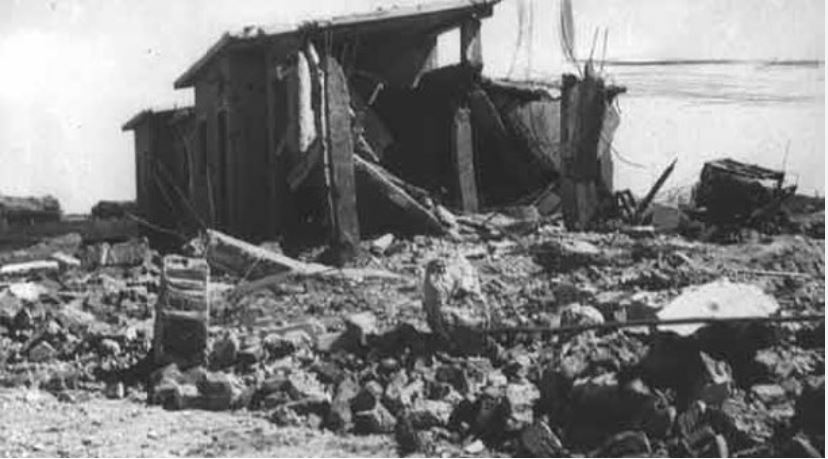
\includegraphics[scale=0.4]{Dolina_2/ByjCq0JSD0Q.jpg}
	%	\label{fig:scipion} % Unique label used for referencing the figure in-text\end{document}
	%	%\addcontentsline{toc}{figure}{Figure \ref{fig:placeholder}} % Uncomment to add the figure to the table of contents%----------------------------------------------------------------------------------------
	\caption{Руины школы в Бахр-эль-Бахр Абу-Забаль. Фото 1}%	CHAPTER 2
\end{figure}

\begin{figure}[h!tb] 
	\centering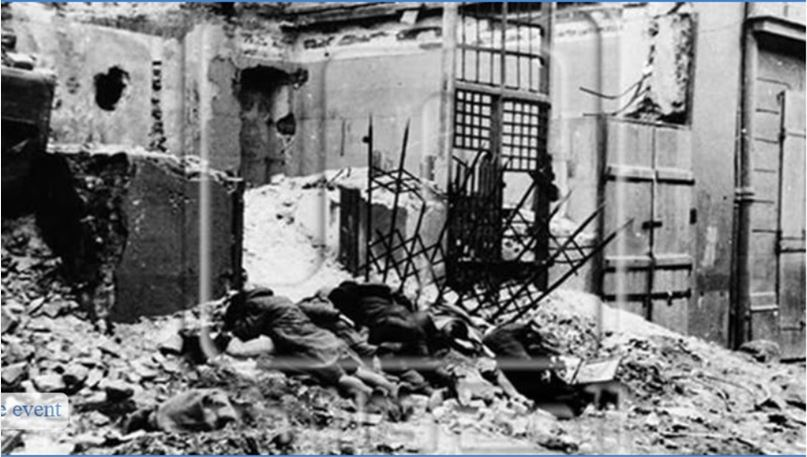
\includegraphics[scale=0.4]{Dolina_2/x-cyre6EBMg.jpg}
	%	\label{fig:scipion} % Unique label used for referencing the figure in-text\end{document}
	%	%\addcontentsline{toc}{figure}{Figure \ref{fig:placeholder}} % Uncomment to add the figure to the table of contents%----------------------------------------------------------------------------------------
	\caption{Руины школы в Бахр-эль-Бахр Абу-Забаль. Фото 2. Оба фото — египетские, так что без гарантий точности.}%	CHAPTER 2
\end{figure}

В феврале и марте, когда израильтяне вовсю бомбили египетские тылы, в Кайро-Уэст прибыла вторая советская авиационная часть - 135-й истребительный авиаполк. Самолёты в прямом смысле прибывали из одного мира в другой - во время погрузки самолётов на Горьковском авиазаводе в грузовой отсек Ан-12 часто попадал снег - в Африке он выглядел настоящим и не очень уместным чудом.

6-го марта прибыли лётчики. Как и их коллег из 35-й ОРЭ, израильтяне подготовили подобающую встречу - в виде пары “Фантомов”, прошедшей на малой высоте. На авиабазе начался страшный бардак - только что прибывшие “специалисты по сельскому хозяйству”, правильно оценив ситуацию, попадали в песок и постарались зарыться в него поглубже. Египтяне устроили дичайшую канонаду (в основном - уже после того, как “Фантомы” улетели) - не столько чтобы кого-то сбить, сколько для успокоения нервов и руководства. В общем, бело-синий комитет по встрече отработал как всегда - шумно и весело. 
135-я авиабригада бригада прикрывала Каир с востока, промышленные объекты центральной части ОАР и Асуанскую плотину с северо-востока. Основные аэродромы базирования - Бени-Суэйф, в 180 км южнее Каира (две эскадрильи), и Ком-Аушим, в 120 км юго-восточнее Каира (эскадрилья). Был ещё запасной аэродром в Заафранской долине — его планировалось использовать по аналогии с Котмией.

Фактически, местность между эль-Сохной и Заафраном - это холмистое плато, изрезанное ущельями, которыми любили пользоваться израильтяне - устойчивая проводка самолёта, летящего на малой высоте в таких условиях была крайне затруднена. А значит - времени отреагировать практически не оставалось. К тому-же, за холмами часто прятались засады “Миражей” и «Фантомов», внезапно в нужный момент появляясь - и исчезая.

Поначалу основной задачей новоприбывших советских лётчиков было прекращение израильских ударов по египетскому тылу - операции “Приха”. Её суть сводилась к следующему - Израиль собирался принудить Египет к прекращению огня, перенеся войну с берегов Суэцкого канала в глубь территории Египта. То есть - навязать египтянам игру по своим правилам, реализуя свои сильные стороны (авиацию) и нивелируя слабые (малочисленную артиллерию).

Впрочем, совсем без инцидентов обойтись не могло — и вот уже в апреле 1970-го группа «Фантомов» была перехвачена МиГами, пилоты которых говорили по-русски …
